\documentclass[11pt,letterpaper]{article}

\usepackage[margin=0.92in,headheight=15pt]{geometry}
\usepackage[T1]{fontenc}
\usepackage[utf8]{inputenc}
\usepackage{lmodern}
\usepackage{microtype}
\usepackage{amsmath,amssymb,amsthm,mathtools}
\usepackage{booktabs,longtable,tabularx,array,multirow}
\usepackage{enumitem}
\usepackage{xcolor}
\usepackage{graphicx}
\usepackage{tikz}
\usetikzlibrary{arrows.meta,positioning,fit,calc,decorations.pathreplacing}
\usepackage[most]{tcolorbox}
\usepackage{listings}
\usepackage{xurl}
\usepackage[hidelinks]{hyperref}
\usepackage[nameinlink,noabbrev]{cleveref}
\usepackage{fancyhdr}
\usepackage{lastpage}
\usepackage{caption}

\definecolor{navy}{HTML}{16324F}
\definecolor{bluegray}{HTML}{EAF0F5}
\definecolor{deepgreen}{HTML}{1F5D42}
\definecolor{palegreen}{HTML}{EAF5EF}
\definecolor{amber}{HTML}{8A5A00}
\definecolor{paleamber}{HTML}{FFF6DF}
\definecolor{deepred}{HTML}{8A2635}
\definecolor{palered}{HTML}{FBECEF}
\definecolor{codebg}{HTML}{F5F7F9}
\definecolor{midgray}{HTML}{5A6670}

\hypersetup{
  pdftitle={Serving Cut Leaves in the forall-PO-Free Fragment of ALCI-RCC5},
  pdfsubject={Candidate repair using support-generated labels and extremal-carrier kernels},
  pdfauthor={OpenAI, prepared from the supplied ALCI-RCC5 packet},
  pdfkeywords={ALCI RCC5, cut leaf, blocking, kernel, Hintikka labels, decidability}
}

\pagestyle{fancy}
\fancyhf{}
\fancyhead[L]{\small\textsc{Cut-Leaf Residue in $\mathsf{ALCI}_{\mathsf{RCC5}}$}}
\fancyhead[R]{\small Candidate construction and proof obligations}
\fancyfoot[L]{\small 26 August 2026}
\fancyfoot[R]{\small Page \thepage\ of \pageref*{LastPage}}
\renewcommand{\headrulewidth}{0.4pt}
\renewcommand{\footrulewidth}{0pt}

\setlist[itemize]{leftmargin=1.35em,itemsep=0.25em,topsep=0.35em}
\setlist[enumerate]{leftmargin=1.6em,itemsep=0.25em,topsep=0.35em}
\setlength{\parindent}{0pt}
\setlength{\parskip}{0.55em}
\setlength{\emergencystretch}{3em}

\newcommand{\ALCIRCC}{\ensuremath{\mathsf{ALCI}_{\mathsf{RCC5}}}}
\newcommand{\DR}{\ensuremath{\mathsf{DR}}}
\newcommand{\PO}{\ensuremath{\mathsf{PO}}}
\newcommand{\EQ}{\ensuremath{\mathsf{EQ}}}
\newcommand{\PP}{\ensuremath{\mathsf{PP}}}
\newcommand{\PPI}{\ensuremath{\mathsf{PPI}}}
\newcommand{\mty}{\operatorname{mty}}
\newcommand{\cl}{\operatorname{cl}}
\newcommand{\sat}{\models}
\newcommand{\MultiTier}{\ensuremath{\mathsf{MultiTier}}}
\newcommand{\MultiTierOk}{\ensuremath{\mathsf{MultiTierOk}}}
\newcommand{\cutNodes}{\ensuremath{\mathsf{cutNodes}}}
\newcommand{\typeEnum}{\ensuremath{\mathsf{typeEnum}}}
\newcommand{\Arg}{\operatorname{Arg}}
\newcommand{\Car}{\operatorname{Car}}
\newcommand{\powerset}{\mathcal{P}}
\newcommand{\code}[1]{\nolinkurl{#1}}

\theoremstyle{definition}
\newtheorem{definition}{Definition}[section]
\newtheorem{construction}[definition]{Construction}
\newtheorem{observation}[definition]{Observation}
\theoremstyle{plain}
\newtheorem{lemma}[definition]{Lemma}
\newtheorem{proposition}[definition]{Proposition}
\newtheorem{theorem}[definition]{Theorem}
\newtheorem{corollary}[definition]{Corollary}
\theoremstyle{remark}
\newtheorem{remark}[definition]{Remark}
\newtheorem{warning}[definition]{Warning}

\newtcolorbox{statusbox}[1][]{
  enhanced,breakable,colback=bluegray,colframe=navy,boxrule=0.6pt,
  arc=1.5mm,left=2mm,right=2mm,top=1.5mm,bottom=1.5mm,#1
}
\newtcolorbox{resultbox}[1][]{
  enhanced,breakable,colback=palegreen,colframe=deepgreen,boxrule=0.7pt,
  arc=1.5mm,left=2mm,right=2mm,top=1.5mm,bottom=1.5mm,#1
}
\newtcolorbox{cautionbox}[1][]{
  enhanced,breakable,colback=paleamber,colframe=amber,boxrule=0.7pt,
  arc=1.5mm,left=2mm,right=2mm,top=1.5mm,bottom=1.5mm,#1
}
\newtcolorbox{researchbox}[1][]{
  enhanced,breakable,colback=palered,colframe=deepred,boxrule=0.7pt,
  arc=1.5mm,left=2mm,right=2mm,top=1.5mm,bottom=1.5mm,#1
}

\lstdefinelanguage{LeanSketch}{
  morekeywords={structure,where,inductive,theorem,lemma,def,noncomputable,open,
    variable,if,then,else,match,with,forall,exists,by,let,in,fun,Prop,Type,Nat,
    Bool,List,Set,Nonempty},
  sensitive=true,
  morecomment=[l]{--},
  morecomment=[s]{/-}{-/},
  morestring=[b]"
}
\lstset{
  basicstyle=\ttfamily\small,
  backgroundcolor=\color{codebg},
  frame=single,
  rulecolor=\color{bluegray},
  breaklines=true,
  columns=fullflexible,
  keepspaces=true,
  showstringspaces=false,
  xleftmargin=0.5em,
  xrightmargin=0.5em,
  aboveskip=0.7em,
  belowskip=0.7em
}

\title{\vspace{-1.5em}\textbf{Serving Cut Leaves in the $\boldsymbol{\forall\PO}$-Free Fragment of \ALCIRCC}\\[0.5em]
\large Support-Generated Labels, Extremal Carriers, and Demand-Carrying Kernels}
\author{Formal technical note prepared from the supplied Lean excerpt and probe packet}
\date{26 August 2026}

\begin{document}
\maketitle

\begin{abstract}
The remaining vertical obligation in the mixed, $\forall\PO$-free fragment of
\ALCIRCC{} concerns a blocking cut leaf whose complete model type repeats an
ancestor's type but whose own $\exists\PP.D$ or $\exists\PPI.D$ witnesses were
not expanded.  Two natural repairs have already failed: recursively expanding
each cut target yields model-prefix-dependent rounds, while borrowing a
blocker's witness through a declared edge collapses to self-witnessing or,
after excluding self-witnesses, performs no work.

This note develops a different candidate route.  First, certificate labels need
not equal complete model types: the literal \MultiTierOk{} obligations permit
support-generated Hintikka labels containing only formulas needed to establish
the root and consequences forced by already-labelled universals.  Second, a
vertical demand admits an order-theoretic dichotomy.  Either its argument has an
extremal carrier, which serves the demand and cannot repeat the same defect, or
there is an infinite chain of carriers of that same argument, from which the
existing recurrence machinery can construct a kernel with demand list
$[D]$.  Consecutive extremal steps in one direction strictly decrease a finite,
formula-derived demand spectrum.

A fixed-formula finite-set fence shows why the distinction matters: the
complete-type external-witness expansion is forced through $2L+1$ model nodes
as the fence length $L$ grows, whereas a two-external, zero-kernel support
certificate suffices for every $L$.  A new negative-control probe checks all non-vacuous
\MultiTierOk{} fields for this thin certificate.  Separate probes find an
extremal carrier for all 305 phase-uncovered residual demands in the supplied
tower suite, with zero carriers repeating the same triggering existential.
These results refute the inference that the measured target-round growth is
inherent to every extraction.  They do \emph{not} yet prove a global
$C_0$-computable bound: support generated by universals and mixed
\PP/\PPI{} alternation remains the decisive open proof obligation.
\end{abstract}

\begin{statusbox}
\textbf{Status and honesty boundary.}
This is a candidate construction and research note, not a proof of general
decidability.  The supplied file \path{lean/EXCERPTS.lean} contains the stated
proof bodies but does not compile standalone because its surrounding
31,783-line development was not supplied.  Accordingly:
\begin{itemize}
  \item \textbf{[C]} means reported Lean-certified in the supplied project and
        inspected in the excerpt, but not independently recompiled here;
  \item \textbf{[M]} means proved mathematically in this note from the stated
        RCC5 order assumptions;
  \item \textbf{[E]} means reproduced by executing a supplied or newly added
        probe with its stated controls;
  \item \textbf{[O]} means open, conjectural, or an implementation interface.
\end{itemize}
The ZIP accompanying this PDF contains the original archive verbatim, all seven
probe sources, fresh outputs, the LaTeX source, and a checksum manifest.
\end{statusbox}

\tableofcontents
\newpage

\section{Problem boundary}

Let $I$ be a strong-equality RCC5 interpretation.  The five role atoms are
$\{\DR,\PO,\EQ,\PP,\PPI\}$, where $\EQ$ is identity, $\PP$ is strict proper
part, and $\PPI$ is its converse.  The fragment forbids formulas
$\forall\PO.C$ but permits $\exists\PO.C$.  The present question concerns only
the vertical $\PP/\PPI$ component of the remaining mixed quadrant.

For a concept $C_0$, write
\[
  \mty_{C_0}^{I}(x)
  = \{F\in\cl(C_0) \mid I,x\sat F\}
\]
for the complete model type used by the supplied extraction.  A certificate
$T : \MultiTier\,\beta\,\kappa$ has external labels
$\tau_E : \beta\to\mathrm{List}(\mathrm{Concept})$, periodic kernel phase
labels, and a quotient RCC5 network.  The structure \MultiTierOk{} records
propositional closure, universal propagation, existential fulfilment, and the
quotient-frame conditions.

The blocking closure \cutNodes{} records complete model types along the current
path.  If a selected witness repeats a type already in the path, the witness is
kept but not recursively expanded.  Such a witness is a \emph{cut leaf}.  It is
therefore present as an external node, yet any existential formulas inherited
from its complete type still require services.

\begin{researchbox}
\textbf{Open residue.}
Given a cut leaf $v$ with
$\exists\PP.D\in\mty_{C_0}^{I}(v)$, place a legitimate service in the
certificate without (i) identifying $v$ with another node, (ii) overriding the
read-off RCC5 frame with an inconsistent declared edge, or (iii) initiating a
number of complete-type expansion rounds controlled by an arbitrary model
prefix rather than by $C_0$.
\end{researchbox}

\section{Certified baseline and failed routes}

\subsection{Reported certified facts}

\begin{longtable}{>{\raggedright\arraybackslash}p{0.28\textwidth}
                  >{\raggedright\arraybackslash}p{0.65\textwidth}}
\toprule
\textbf{Lean name} & \textbf{Consequence used in this note} \\
\midrule
\endfirsthead
\toprule
\textbf{Lean name} & \textbf{Consequence used in this note} \\
\midrule
\endhead
\code{odOfModel}, \code{odNet_frame} &
The model's own $\PP$ and $\DR$ relations form an order/disjointness structure,
and its induced RCC5 network is composition-closed. [C] \\
\code{cutNodes_stable_typeEnum} &
The current blocking closure stabilises at fuel $|\typeEnum(C_0)|$ for every
witness selector.  This proves termination of one closure pass, not service of
cut leaves. [C] \\
\code{cutNodes_up_mem}, \code{cutNodes_dn_mem} &
Every vertical witness selected for an expanded node is present in the closure,
including a witness retained as a cut. [C] \\
\code{readoff_ee_all_pp}, \code{readoff_ee_all_ppi},
\code{readoff_ee_all_dr} &
Under read-off relations, external universal propagation follows from model
truth and the frame. [C] \\
\code{readoff_e_ex_pp}, \code{readoff_e_ex_ppi} &
Vertical external existential fulfilment reduces to membership of a genuine
model witness in the selected set or in a serving kernel phase. [C] \\
\code{chain_or_kernel}, \code{rr_covers} &
An arbitrary ascending demand-following chain either terminates or yields a
kernel; persistent demand lists can be covered round-robin.  The supplied
\code{chain_or_kernel} builds \code{KernelData} with an empty demand list. [C] \\
\bottomrule
\end{longtable}

These facts sharply isolate the issue.  With read-off relations, adding a real
model point preserves the RCC5 frame and makes universal propagation truthful.
The unresolved question is which real points, kernels, or regular occurrences
must be represented finitely.

\subsection{Why the two rejected answers remain rejected}

\paragraph{Complete-type target expansion.}
Probe \code{wp116_target_rounds.py} adds and expands targets for unresolved cut
leaves.  With period fixed at three, the reproduced maximum round count grows
with the aperiodic prefix:

\begin{center}
\begin{tabular}{rrrrrrr}
\toprule
Prefix $L$ & 4 & 8 & 12 & 18 & 26 & 40 \\
\midrule
Maximum rounds & 3 & 5 & 6 & 9 & 12 & $\geq 15$ \\
\bottomrule
\end{tabular}
\end{center}

At $L=40$, 19 runs hit the ceiling, so 15 is only a lower bound.  The control
requiring an unresolved round-zero cut leaf was positive in every shape. [E]
This refutes a bound for that extraction strategy based solely on repeated
complete types.

\paragraph{Declared-edge borrowing.}
The historical declared-edge treatment achieved apparent 100\% coverage only
by allowing a cut leaf to be its own witness.  Once $w\neq v$ is enforced, the
305 phase-uncovered cases have no already-selected edge witness; all 305 require
a new model point.  In the current \code{wp118_multitier_acceptance.py}, declared
edges ON and OFF produce exactly the same failures:
\[
  e\_ex\_\PP=37,\qquad k\_ex\_\PP=42,\qquad k\_ex\_\PPI=336.
\]
Thus the guarded treatment performs no work in the kernel-bearing class. [E]

\begin{warning}
The reproduced \code{wp117} banner still states that its redesign has an answer,
but the same output reports ``witness is a NEW node: 305.''  The banner is a
retired conclusion, not evidence.  The accompanying package preserves this
verbatim so the inconsistency remains auditable.
\end{warning}

\section{The architectural slack: labels need not be complete types}

\begin{observation}[No full-type axiom in \MultiTierOk]\label{obs:no-full-type}
The literal definition of \MultiTierOk{} contains no field asserting
\[
   \tau_E(e)=\mty_{C_0}^{I}(e)
   \quad\text{or}\quad
   \mathsf{phase}(k,a)=\mty_{C_0}^{I}(x_{k,a}).
\]
Its obligations are conditional on formulas that actually occur in the
certificate labels.
\end{observation}

\begin{proof}
Inspection of the supplied structure shows only clash-freedom, absence of
bottom, Boolean decomposition, universal propagation, and existential
fulfilment for labelled formulas, together with the quotient-frame condition.
There is neither a maximality clause nor a requirement to list every true
subformula of $C_0$.
\end{proof}

This observation does not itself produce a certificate.  It identifies an
unnecessary extraction invariant: the current construction equates a
certificate label with the complete set of all true closure formulas, including
true formulas beneath disjuncts that were not chosen to support $C_0$.

\subsection{Support-generated labels}

\begin{construction}[Model-guided support saturation]\label{con:support}
Maintain a finite or regular collection of external occurrences and kernel
phase occurrences.  Associate each occurrence $u$ with a support label
$\Gamma(u)\subseteq\cl(C_0)$.  Seed the root occurrence $u_0$ with $C_0$, and
close under the following rules.

\begin{enumerate}
  \item If $C\sqcap D\in\Gamma(u)$, add both $C$ and $D$ to $\Gamma(u)$.
  \item If $C\sqcup D\in\Gamma(u)$, add one disjunct true at the model point
        represented by $u$.
  \item If $\forall r.C\in\Gamma(u)$ and the certificate's read-off relation
        from $u$ to $v$ is $r$, add $C$ to $\Gamma(v)$.  The analogous rules
        are applied to all external/kernel edge classes required by
        \MultiTierOk{}.
  \item If $\exists r.C\in\Gamma(u)$, record one legal service branch and add
        $C$ to the serving external or phase label.
\end{enumerate}
No other true formula is inserted merely because it belongs to the represented
model point's complete type.
\end{construction}

\begin{lemma}[Truth invariant]\label{lem:truth-invariant}
Assume every external service is a genuine model witness, every relation is
read off from the model, every disjunction chooses a model-true disjunct, and
every kernel phase is represented by a model point on its witnessing chain.
Then support saturation preserves
\[
   F\in\Gamma(u) \quad\Longrightarrow\quad I,x_u\sat F.
\]
\end{lemma}

\begin{proof}
Induct over insertions.  The root seed is true by hypothesis.  Conjunction and
disjunction insertions preserve truth by their semantics.  For a universal,
read-off relation $r$ and truth of $\forall r.C$ at the source imply truth of
$C$ at the target.  For an existential, the chosen service is required to be a
real $r$-successor satisfying its argument.  The kernel case uses the model
points that witness the kernel phases.
\end{proof}

\begin{proposition}[Conditional obligation discharge]\label{prop:conditional-ok}
Suppose support saturation terminates in a finite multi-tier object, the
quotient network is a read-off \code{odNet}, and every labelled existential has
a recorded legal service branch.  Then the resulting labels satisfy the
propositional, universal, and existential fields of \MultiTierOk{}.
\end{proposition}

\begin{proof}
The Boolean fields hold by saturation rules 1--2.  The universal fields hold by
rule 3 for each edge class.  The existential fields hold by rule 4 and the
recorded service branch.  The frame field is supplied independently by the
read-off order/disjointness construction.  Kernel period positivity and phase
well-formedness remain explicit construction side conditions.
\end{proof}

\begin{cautionbox}
\textbf{What this changes, and what it does not.}
A new witness may still be added as a distinct external node.  The difference
from target-round expansion is that the node receives only the demanded
argument and forced support consequences, not its complete model type.  The
open theorem is therefore termination or regular representability of the
\emph{support-generated} service graph, not termination of repeated complete
model-type expansion.
\end{cautionbox}

\section{Extremal carrier or demand-carrying kernel}

The second component changes witness selection.  It is order-theoretic and does
not rely on type repetition.

\begin{definition}[Ascending carrier set]
For a demand $\exists\PP.D$ true at $x$, define
\[
  \Car_D^+(x)
  =\{y \mid x<y,\ I,y\sat D\},
\]
where $x<y$ abbreviates $I.\rho(x,y)=\PP$.  A member $y$ is
$D$-\emph{maximal} if no $z\in\Car_D^+(x)$ satisfies $y<z$.
\end{definition}

\begin{theorem}[Extremal carrier or $D$-chain]\label{thm:dichotomy}
Let $<$ be the strict transitive $\PP$ order of an RCC5 interpretation.  If
$I,x\sat\exists\PP.D$, then the following case distinction is available:
\begin{enumerate}
  \item there is a $D$-maximal $y\in\Car_D^+(x)$; or
  \item there is a sequence $c:\mathbb{N}\to\Delta^I$ with $c(0)=x$,
        $c(n)<c(n+1)$ for all $n$, and $I,c(n)\sat D$ for every $n\geq 1$.
\end{enumerate}
The displayed outcomes can coexist in a branching order: a model may contain
both a maximal carrier and a separate infinite carrier branch.  The construction
uses the first outcome whenever a maximal carrier exists and invokes the chain
construction only under the negation of that existence claim.
\end{theorem}

\begin{proof}
The carrier set is nonempty by the existential semantics.  If it has a maximal
member, choose it.  Otherwise every $D$-carrier above $x$ has a strictly higher
$D$-carrier.  Choose $c(1)\in\Car_D^+(x)$; then use dependent choice to select
$c(n+1)$ above $c(n)$ while preserving $D$.  Set $c(0)=x$.  Strict transitivity
keeps every later point above $x$.
\end{proof}

\begin{figure}[ht]
\centering
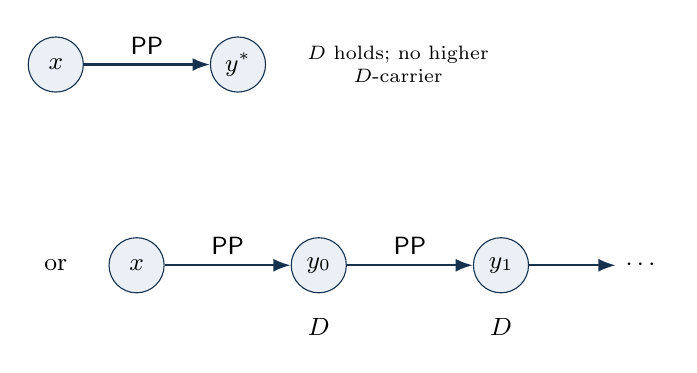
\begin{tikzpicture}[
  node distance=13mm and 16mm,
  every node/.style={font=\small},
  point/.style={circle,draw=navy,fill=bluegray,minimum size=7mm,inner sep=1pt},
  darr/.style={-{Latex[length=2.2mm]},thick,draw=navy}
]
\node[point] (x1) {$x$};
\node[point,right=of x1] (ym) {$y^*$};
\draw[darr] (x1) -- node[above] {$\PP$} (ym);
\node[align=center,right=4mm of ym] {\scriptsize $D$ holds; no higher\\[-1mm]\scriptsize $D$-carrier};

\node[below=20mm of x1] (or) {or};
\node[point,right=4mm of or] (x2) {$x$};
\node[point,right=of x2] (y0) {$y_0$};
\node[point,right=of y0] (y1) {$y_1$};
\node[right=11mm of y1] (dots) {$\cdots$};
\draw[darr] (x2) -- node[above] {$\PP$} (y0);
\draw[darr] (y0) -- node[above] {$\PP$} (y1);
\draw[darr] (y1) -- (dots);
\node[below=2mm of y0] {$D$};
\node[below=2mm of y1] {$D$};
\end{tikzpicture}
\caption{Carrier-specific dichotomy for a demand $\exists\PP.D$.}
\end{figure}

\begin{lemma}[An extremal target drops the same defect]\label{lem:drop}
If $y$ is a $D$-maximal member of $\Car_D^+(x)$, then
$I,y\not\sat\exists\PP.D$.
\end{lemma}

\begin{proof}
Otherwise existential semantics provides $z$ with $y<z$ and $I,z\sat D$.
Transitivity gives $x<z$, so $z\in\Car_D^+(x)$, contradicting maximality.
\end{proof}

\begin{proposition}[Demand-carrying kernel from the non-extremal branch]
\label{prop:d-kernel}
Assume the supplied recurrence theorem \code{kernel_of_chain}.  From the second
branch of \cref{thm:dichotomy}, one can construct
\[
  \mathsf{KernelData}\ I\ C_0\ [D]\ L_0\ \mathsf{true}\ x.
\]
In particular, the kernel's \code{ccovers} field is discharged without a
persistence guard.
\end{proposition}

\begin{proof}
Apply the existing chain recurrence theorem to $c$ and choose its returned
indices $i>0$ and $p>0$.  Copy the domain, step, root, base, positivity, and
repeated-type fields into \code{KernelData}.  For the sole demand $D\in[D]$,
choose phase offset $b=0$.  Since $i>0$, the construction of $c$ gives
$I,c(i)\sat D$, hence $D\in\mty_{C_0}^{I}(c(i+0))$, and $0<p$.  Thus
\code{ccovers} holds.  No round-robin persistence assumption is needed because
every positive chain point carries $D$.
\end{proof}

The descending mirror uses the converse strict order and produces a descending
$D$-carrying kernel for $\exists\PPI.D$.  The excerpt explicitly notes that the
current \code{chain_or_kernel} theorem is ascending only, so its Lean mirror is
a separate formalization task. [O]

\subsection{A finite one-direction rank}

Let
\[
  \Arg_{\PP}(C_0)=\{D\mid \exists\PP.D\in\cl(C_0)\}
\]
and define the ascending demand spectrum
\[
  U(x)=\{D\in\Arg_{\PP}(C_0)\mid I,x\sat\exists\PP.D\}.
\]

\begin{lemma}[Monotonicity and strict extremal descent]\label{lem:spectrum}
If $x<y$, then $U(y)\subseteq U(x)$.  If, in addition, $y$ is selected as a
$D$-maximal carrier for a demand $D\in U(x)$, then
$U(y)\subsetneq U(x)$.
\end{lemma}

\begin{proof}
For $E\in U(y)$, choose $z$ with $y<z$ and $I,z\sat E$.  Transitivity yields
$x<z$, so $E\in U(x)$.  For strictness, \cref{lem:drop} gives $D\notin U(y)$
while $D\in U(x)$.
\end{proof}

\begin{corollary}[Bound on consecutive extremal ascending services]
Any sequence in which every step is an extremal $\PP$ service has length at
most $|\Arg_{\PP}(C_0)|$.  The descending mirror is bounded by
$|\Arg_{\PPI}(C_0)|$.
\end{corollary}

\begin{warning}
This is not yet a global rank.  A $\PP$ step may enlarge the downward demand
spectrum, and a later $\PPI$ step may enlarge the upward spectrum.  Mixed
alternation can therefore evade a simple lexicographic combination.  Support
labels remove demands that arose only from complete-type overlabelling, but a
proof is still needed for alternation generated by formulas genuinely in the
support.
\end{warning}

\section{A fixed-formula fence separating complete types from support}

This family gives a concrete model-normalisation witness: the same $C_0$ admits
arbitrarily long satisfying models on which complete-type expansion grows, yet
also admits a constant-size certificate extracted from each model.

\subsection{Finite-set RCC5 model}

Fix a common element $c$.  For $0\leq i\leq L$, let
\[
  X_i=\{c,x_i\},
\]
and for $0\leq i<L$, let
\[
  Y_i=\{c,x_i,x_{i+1},y_i\}.
\]
RCC5 relations are derived from set semantics.  Thus
$X_i\PP Y_i$ and $X_{i+1}\PP Y_i$; all other distinct pairs not forced by
these inclusions overlap properly.

Use atoms $R,A_0,A_1,B_0,B_1$.  Make $R$ true only at $X_0$, alternate
$A_0,A_1$ over the $X_i$, and alternate $B_0,B_1$ over the $Y_i$.  Define
\[
\begin{aligned}
F_0&=\exists\PP.B_0, & F_1&=\exists\PP.B_1,\\
G_0&=\exists\PPI.A_1, & G_1&=\exists\PPI.A_0,\\
J&=F_1\sqcap(G_0\sqcap G_1),\\
C_0&=F_0\sqcap(R\sqcup J).
\end{aligned}
\]
This fixed concept is $\forall\PO$-free.  It is a vertical stress test rather
than a complete mixed-quadrant example, because it contains no
$\exists\PO$ demand.

\begin{figure}[ht]
\centering
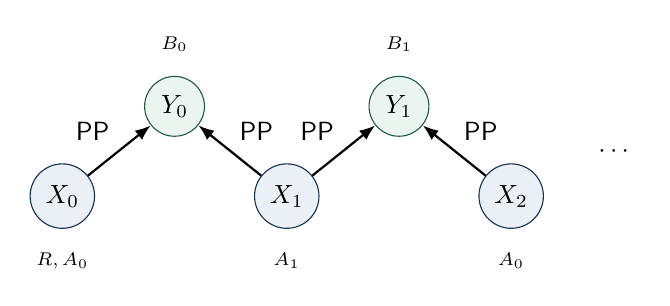
\begin{tikzpicture}[
  xnode/.style={circle,draw=navy,fill=bluegray,minimum size=8mm},
  ynode/.style={circle,draw=deepgreen,fill=palegreen,minimum size=8mm},
  arr/.style={-{Latex[length=2mm]},thick},
  scale=0.95,transform shape
]
\node[xnode] (x0) at (0,0) {$X_0$};
\node[ynode] (y0) at (1.5,1.2) {$Y_0$};
\node[xnode] (x1) at (3,0) {$X_1$};
\node[ynode] (y1) at (4.5,1.2) {$Y_1$};
\node[xnode] (x2) at (6,0) {$X_2$};
\node at (7.4,0.6) {$\cdots$};
\draw[arr] (x0) -- node[above left] {$\PP$} (y0);
\draw[arr] (x1) -- node[above right] {$\PP$} (y0);
\draw[arr] (x1) -- node[above left] {$\PP$} (y1);
\draw[arr] (x2) -- node[above right] {$\PP$} (y1);
\node[below=2mm of x0] {\scriptsize $R,A_0$};
\node[above=2mm of y0] {\scriptsize $B_0$};
\node[below=2mm of x1] {\scriptsize $A_1$};
\node[above=2mm of y1] {\scriptsize $B_1$};
\node[below=2mm of x2] {\scriptsize $A_0$};
\end{tikzpicture}
\caption{The alternating finite-set fence used by probes \code{wp120} and
\code{wp121}.  Arrow direction denotes proper-part inclusion.}
\end{figure}

\begin{proposition}[Complete-type external-witness expansion traverses the fence]
Any read-off closure over the displayed finite model that labels each selected
external with its complete $C_0$-model type and fulfils every labelled vertical
existential by a genuine external model witness must select all $2L+1$ fence
points.
\end{proposition}

\begin{proof}
At $X_0$, $F_0$ is true and its only $B_0$-carrying proper superregion is
$Y_0$, so $Y_0$ is selected.  At $Y_0$, both $G_0$ and $G_1$ are true because
its proper subregions $X_0$ and $X_1$ carry the two alternating $A$ atoms; hence
$X_1$ is selected.  Inductively, once $X_i$ is selected, the appropriate
$F_0$ or $F_1$ in its complete type forces the previously unselected $Y_i$;
then the two $G$ formulas at $Y_i$ force $X_{i+1}$.  Thus every $X_i$ and $Y_i$
is selected.
\end{proof}

\begin{proposition}[Constant-size support certificate]\label{prop:two-node}
For every $L\geq 1$, the same model contains a two-external, zero-kernel
certificate with labels
\[
\begin{aligned}
\Gamma(X_0)&=\{C_0,F_0,R\sqcup J,R\},\\
\Gamma(Y_0)&=\{B_0\},
\end{aligned}
\]
and read-off relation $E(X_0,Y_0)=\PP$.
\end{proposition}

\begin{proof}
The root conjunction is decomposed into $F_0$ and $R\sqcup J$; the true
left disjunct $R$ is selected.  The sole labelled existential $F_0$ is served
by the distinct point $Y_0$, whose label contains $B_0$.  There are no labelled
universals and no other labelled existentials.  The two-point read-off network
is an induced subnetwork of the finite-set RCC5 model, so identity, converse,
and composition constraints hold.  All kernel obligations are vacuous.
\end{proof}

\subsection{Measured separation and full-obligation control}

\begin{center}
\begin{tabular}{rrrrr}
\toprule
$L$ & Model nodes & Complete-type rounds & Complete-type nodes & Support nodes \\
\midrule
4  & 9  & 2  & 9  & 2 \\
8  & 17 & 4  & 17 & 2 \\
12 & 25 & 5  & 25 & 2 \\
18 & 37 & 8  & 37 & 2 \\
26 & 53 & 11 & 53 & 2 \\
40 & 81 & 16 & 81 & 2 \\
\bottomrule
\end{tabular}
\end{center}

Probe \code{wp121_support_multitier_acceptance.py} then checks every
non-vacuous field of \MultiTierOk{} for the two-node certificate: quotient-frame
identity/converse/composition, \code{e_clash}, \code{e_nobot}, \code{e_and},
\code{e_or}, \code{ee_all}, and \code{e_ex}.  For each
$L\in\{1,2,4,8,12,18,26,40\}$, removing $B_0$ from $Y_0$ yields exactly one
\code{e_ex} failure, while restoring it yields no failures. [E]

\begin{resultbox}
The fence is a formal counterexample to the inference
``unbounded complete-type target rounds for a fixed formula imply that every
certificate extraction for that formula is unbounded.''  It is not a proof
that support generation is always finite; it isolates complete-type
\emph{overlabelling} as one genuine source of spurious model-length growth.
\end{resultbox}

\section{Probe evidence and its exact force}

All seven probes were executed from a clean extracted copy of the supplied
archive.  The fresh logs are included in \path{outputs/reproduced/}.

\begin{longtable}{>{\raggedright\arraybackslash}p{0.18\textwidth}
                  >{\raggedright\arraybackslash}p{0.35\textwidth}
                  >{\raggedright\arraybackslash}p{0.38\textwidth}}
\toprule
\textbf{Probe} & \textbf{Reproduced observation} & \textbf{Permitted conclusion} \\
\midrule
\endfirsthead
\toprule
\textbf{Probe} & \textbf{Reproduced observation} & \textbf{Permitted conclusion} \\
\midrule
\endhead
\code{wp112} &
Tail continuation 94.0--99.4\%; prefix 33.2--55.6\% by shape; side 0\%.
Control failures: 0. &
An arbitrary blocked lap often, but not always, continues.  Side leaves cannot
be repaired by ``continue the same chain.'' \\
\code{wp115} &
Finite read-off certificates pass with declared edges ON and have 37 vertical
failures with edges OFF. &
The finite model class exercises read-off obligations but cannot validate
kernel interactions.  Its edge result was superseded. \\
\code{wp116} &
Maximum complete-type target rounds grow from 3 to at least 15 as $L$ grows
from 4 to 40. &
That extraction's round bound is model-prefix-dependent.  No conclusion about
all possible certificates follows. \\
\code{wp117} &
Phase-or-edge coverage prints 100\%, but all 305 edge-only witnesses are new
nodes. &
Phase coverage is useful; the final ``no new node'' banner is invalid and is
retired. \\
\code{wp118} &
Declared edges ON and OFF have identical $e\_ex/k\_ex$ failures in a
kernel-bearing class. &
After excluding self-witnesses, the declared-edge treatment does no work. \\
\code{wp119} &
All 305 phase-uncovered demands have an extremal carrier; 0 targets repeat the
same triggering existential.  Random tower sweeps select at most 5 externals
and depth at most 3, with controls holding. &
Extremal selection defeats the measured prefix effect in this tower class.  It
is not a \MultiTierOk{} acceptance test and does not settle mixed alternation. \\
\code{wp120}/\code{wp121} &
For the fixed fence, complete types select $2L+1$ points while support uses 2;
negative control fails and the treatment passes all applicable obligations. &
Thin labels are architecturally legitimate for this family.  General support
termination remains open. \\
\bottomrule
\end{longtable}

\subsection{The 305-demand residue}

The exact phase-uncovered residue revisited by \code{wp119} is:

\begin{center}
\begin{tabular}{lr}
\toprule
Residual property & Count \\
\midrule
Residual demands & 305 \\
Has an extremal $D$-carrier & 305 \\
Extremal carrier already selected & 0 \\
Extremal carrier is a new real node & 305 \\
Target repeats $\exists r.D$ & 0 \\
No extremal carrier & 0 \\
\bottomrule
\end{tabular}
\end{center}

This does not mean that the new target has no other obligations under a complete
model type.  It means that the target is terminal for the \emph{same signed
demand}.  Support labels are what prevent unrelated complete-type obligations
from restarting the old round mechanism.

\subsection{Fixed-formula extremal control}

With $C_0=\exists\PP.A$ fixed while only the irrelevant tower prefix grows,
\code{wp119} reports:

\begin{center}
\begin{tabular}{rrrrr}
\toprule
$L$ & Nearest-witness rounds & Extremal externals & Depth & Kernels \\
\midrule
4  & 2  & 2 & 1 & 0 \\
8  & 4  & 2 & 1 & 0 \\
12 & 6  & 2 & 1 & 0 \\
18 & 9  & 2 & 1 & 0 \\
26 & 13 & 2 & 1 & 0 \\
40 & 20 & 2 & 1 & 0 \\
\bottomrule
\end{tabular}
\end{center}

This is an explicit model-normalisation pattern: select a far extremal carrier
rather than accepting the model's nearest-witness prefix.

\section{Proposed extraction interface}

The current selector always returns a model node, after which \cutNodes{}
recurses over every vertical existential in its depth-bounded complete type.
The proposed selector returns a \emph{service} and the closure operates on
support labels.

\begin{lstlisting}[language=LeanSketch,caption={Lean-style interface sketch; not compiled.}]
inductive VerticalService (I : Interp alpha) (C0 : Concept)
  | external
      (y : alpha)                  -- genuine, distinct model point
      (hy : I.dom y)
      (edge : Atom)                -- read off from I.rho
      (seed : List Concept)        -- normally [D], then saturated
  | kernel
      (D : Concept)
      (K : KernelData I C0 [D] L0 direction root)

structure SupportOccurrence where
  point    : ModelPointOrPhase
  incoming : Option Atom
  parent   : Option SupportProfile
  label    : Finset Concept
\end{lstlisting}

\subsection{Worklist construction}

\begin{enumerate}
  \item Start with one root occurrence labelled $\{C_0\}$.
  \item Saturate Boolean rules and all universal consequences along the current
        read-off quotient network.
  \item For each unserved vertical $\exists r.D$ in a support label:
    \begin{enumerate}[label=(\alph*)]
      \item reuse an already selected genuine target when it serves the demand;
      \item otherwise choose an $r$-extremal $D$-carrier and add it with seed
            $\{D\}$;
      \item if no extremal carrier exists, insert an $r$-directed kernel whose
            demand list is $[D]$.
    \end{enumerate}
  \item Re-saturate because a new read-off node can create new targets for
        already-labelled universals.
  \item Continue until no obligation is new, or replace a repeated support
        profile by an explicitly justified regular service object.
\end{enumerate}

\subsection{Non-negotiable invariants}

\begin{itemize}
  \item \textbf{Truth:} every label remains a subset of the represented model
        point's complete type.
  \item \textbf{Read-off frame:} no declared override changes the model's RCC5
        relation; \code{odOfModel}/\code{odNet_frame} remain applicable.
  \item \textbf{No identity collapse:} an external witness is a distinct
        occurrence and, where required, a distinct model point; no node serves a
        strict $\PP/\PPI$ demand with itself.
  \item \textbf{Service provenance:} each existential stores the exact
        \MultiTierOk{} branch that fulfils it.
  \item \textbf{Control before treatment:} every acceptance probe includes a
        mutation that must fail the targeted obligation.
\end{itemize}

\section{What remains to prove}

The proposal reduces the open question but does not eliminate it.  The following
milestones are ordered from local and likely straightforward to global and
high-risk.

\begin{enumerate}
  \item \textbf{Carrier dichotomy in Lean.}  Formalise
        \cref{thm:dichotomy} for $\PP$, using the existing existential witness
        lemmas and classical choice. [M $\rightarrow$ C]
  \item \textbf{$[D]$ kernel constructor.}  Wrap the existing chain recurrence
        theorem and prove \code{ccovers} with offset zero, as in
        \cref{prop:d-kernel}. [M $\rightarrow$ C]
  \item \textbf{Descending mirror.}  Repeat for $\PPI$ or transport through the
        converse order, matching the project's descending kernel definitions.
        [O]
  \item \textbf{Support truth and saturation.}  Define finite support labels and
        prove \cref{lem:truth-invariant} for every external/kernel edge class.
        [M $\rightarrow$ C]
  \item \textbf{Support-to-\MultiTierOk{} theorem.}  Show that a saturated,
        service-complete support object induces the literal obligation fields,
        including \code{ek_all}, \code{ke_all}, \code{kk_pp},
        \code{kk_ppi}, \code{kq_all}, and \code{k_ex}. [O]
  \item \textbf{Global regularity theorem.}  Prove that the support-generated
        service graph is bounded by a computable function of $C_0$, or that every
        repeated support context can be compiled into the existing kernel/Q
        architecture.  This is the decisive unresolved step. [O]
  \item \textbf{Mixed-direction stress suite.}  Add adversarial formulas in
        which universals deliberately regenerate alternating $\PP$ and $\PPI$
        existentials.  The treatment must be withheld unless a negative control
        demonstrates that the probe can observe a missing cross-direction
        service. [O]
\end{enumerate}

\subsection{Likely finite state, and why it may still be insufficient}

A plausible blocking state is not a complete model type alone but a contextual
support profile
\[
  \Pi(u)=
  \bigl(\Gamma(u),\Gamma(\operatorname{parent}(u)),r_{\mathrm{in}},
        B_{\PP}(u),B_{\PPI}(u)\bigr),
\]
where $B_{\PP}$ and $B_{\PPI}$ record active box consequences.  There are
computably many such profiles over $\cl(C_0)$.  Standard pairwise blocking
intuition suggests that a repeated monotone profile should admit regular
unfolding.  RCC5 composition and total pairwise relations make that intuition
insufficient by itself: a proof must show that replacing the repeated suffix
preserves every quotient-frame relation to existing externals and kernels.

If the existing linear kernels cannot encode a non-monotone repeated profile,
a precise fallback is an explicit \emph{bud/backpointer} service whose semantics
is a fresh-copy unfolding, not identity in the finite quotient.  This would
answer the user's option (3), but it extends the certificate architecture and
therefore requires a new soundness theorem. [O]

\section{Decisive positive and negative outcomes}

A positive result needs a theorem of the following shape.

\begin{researchbox}
\textbf{Target completeness theorem.}
There is a computable function $B$ such that, whenever a $\forall\PO$-free
concept $C_0$ is satisfiable, there exists a finite support-generated
\MultiTier{} certificate $T$ with a root $e_0$, $C_0\in\tau_E(e_0)$,
\MultiTierOk$(T)$, and
\[
  |\beta|+\sum_{k\in\kappa}p(k)\leq B(C_0).
\]
The certificate uses read-off RCC5 relations and serves each vertical demand by
an existing target, an extremal thin external, or a demand-carrying kernel.
\end{researchbox}

A route-killing counterexample would instead be a satisfiable fixed $C_0$ for
which every certificate in the unchanged external-plus-linear-kernel
architecture requires unboundedly many support-distinct external occurrences
or kernels.  To be decisive, such a family must quantify over witness choices
and thin labels, not merely over nearest-witness or complete-type extraction.

\section{Conclusion}

The strongest current diagnosis is that the cut-leaf question is partly posed
at the wrong abstraction level.  A cut leaf owes every demand in its complete
model type only because the extraction chose complete model types as certificate
labels.  The certificate definition itself asks for a supported Hintikka label,
not a maximal one.

The most promising repair is therefore the combination:
\[
  \boxed{\text{support-generated labels}}
  \quad+\quad
  \boxed{\text{extremal $D$-carrier or $D$-carrying kernel}}.
\]
The first component removes obligations introduced solely by true but unused
closure formulas.  The second bypasses arbitrary model prefixes and ensures
that an extremal target cannot repeat the same signed demand.  A finite,
formula-derived rank bounds consecutive extremal moves in either one direction.
The fixed fence and the 305-demand residue both support this diagnosis, and the
new full-obligation negative-control probe validates the thin certificate on an
adversarial family.

The remaining hard question is no longer ``how does a complete-type cut leaf
serve all demands inherited from its model point?''  It is:

\begin{quote}
\emph{Can every support-generated, mixed-direction recurrence be represented by
finitely many externals and the current periodic kernels, with a bound computable
from $C_0$?}
\end{quote}

That is a materially narrower and more falsifiable theorem than the original
target-round problem.

\appendix
\section{Lean proof targets}

The package contains \path{candidates/lean/CANDIDATE_LEMMAS.lean}, a commented
interface sketch.  The central intended statement is:

\begin{lstlisting}[language=LeanSketch]
theorem pp_carrier_extremal_or_covering_kernel
    (hI : RCC5Interp I) (C0 : Concept) (L0 : Nat)
    (x : alpha) (hx : I.dom x) (D : Concept)
    (hD : Concept.ex pp D in mty C0 I x) :
  (exists y,
      I.dom y /\ I.rho x y = pp /\ D in mty C0 I y /\
      forall z, I.dom z -> I.rho y z = pp -> D notin mty C0 I z)
  \/ Nonempty (KernelData I C0 [D] L0 true x)
\end{lstlisting}

The exact syntax must be adapted to the full development's witness lemmas and
list-membership notation.  No claim is made that this sketch compiles.

\section{Reproduction}

From the unpacked project root:

\begin{lstlisting}[language=bash]
cd original/probes
python3 wp112_lap_continuation_closed_form.py
python3 wp115_declared_edge_acceptance.py
python3 wp116_target_rounds.py
python3 wp117_kernel_phase_coverage.py
python3 wp118_multitier_acceptance.py

cd ../../candidates/probes
python3 wp119_extremal_carrier_probe.py
python3 wp120_support_label_fence.py
python3 wp121_support_multitier_acceptance.py
\end{lstlisting}

The convenience script \path{scripts/run_all_probes.sh} sets the required
\code{PYTHONPATH} so the candidate probes can import the original tower code.
The file \path{MANIFEST.sha256} records checksums for the packaged artifacts.

\end{document}
